\documentclass[12pt,oneside,openright]{report}

\usepackage[utf8]{inputenc}
\usepackage[scaled]{helvet}
\usepackage{subcaption} % Add the subcaption package for subfigures
\usepackage{dirtytalk} %quoting package
\renewcommand\familydefault{\sfdefault} 
\usepackage[T1]{fontenc}
\usepackage{fancyhdr,xcolor}

\usepackage{graphicx} % Add the graphicx package for including images
\usepackage{geometry}
\usepackage{amsmath} % Add this line to your LaTeX preamble to use \text

\usepackage{pdfpages}
\usepackage{afterpage}
\usepackage{caption}
\usepackage{float}
\usepackage{xcolor}
\usepackage[style=authoryear,backend=biber]{biblatex}
\addbibresource{bibliog.bib}
\usepackage[colorlinks=true,linkcolor=black,anchorcolor=black,citecolor=black,filecolor=black,menucolor=black,runcolor=black,urlcolor=black]{hyperref}\usepackage{graphicx}
\geometry{
  a4paper,
  left=20mm,
  right=20mm,
  top=3cm,
  headheight=4cm,
  bottom=3.5cm,
  footskip=3cm
}

\renewcommand*{\bibfont}{\footnotesize}

\newcommand{\changefont}{
    \fontsize{18}{16}\selectfont
}
\definecolor{boxcl}{HTML}{1188BB}
\definecolor{tubred}{HTML}{1188BB}



\begin{document}

\begin{titlepage}
    \centering
    % Include the image with a width of one-third of the page
    
\includegraphics[width=0.5\textwidth]{Hu-logo.png}
    \vspace{2cm}
    
    {\huge \textbf{Multisensory Integration in Virtual Reality: Effects of Passive Haptic Stimulation}\par}
    \vspace{2cm}
    {\LARGE Master Thesis\par}
    \vspace{0.5cm}
    {\textbf{submitted in fulfillment of the requirements for the degree}\par}
    Master of Science (M.Sc.)\par
    {\textbf{in the master's program ``Mind and Brain''}\par}
    \vspace{1.5cm}
    {\textbf{Humboldt-Universität zu Berlin}\par}
    {\textbf{Berlin School of Mind and Brain}\par}
    \vfill
    \raggedright
    \begin{tabular}{ll}
        \textbf{Handed in by}: & Benjamin Dupré \\
        \textbf{Date of birth:} & 26.04.1986\\
       \textbf{ Address:} & Hoppestraße 16, 13409, Berlin \\
    \end{tabular}
    \vfill
    \begin{tabular}{ll}
        \textbf{1. Supervisor:}& Dr. Michael Gaebler \\
        \textbf{2. Supervisor:}& Professor Dr. Arno Villringer  \\
    \end{tabular}
    \vfill
    {Berlin, \today \par}
\end{titlepage}

\section*{1. Introduction}
\subsection*{1.1 Problem \& Significance}

We have all heard at some point that our body behaves like an orchestra, with the brain as the conductor. Within this orchestra, multiple specialized musicians coordinate, together creating a melody grander than any individual musician could aspire to achieve alone. The brain serves as an orchestra director, managing and coordinating various bodily functions. However, as proposed by \cite{Morten2021}, it's more plausible that the brain isn't merely a single orchestra coordinator but rather a team of orchestra coordinators. Recent findings suggest an unseen conductor outside the brain, providing subtle cues that dictate whether the symphony focuses on its harmonies or the audience's mood. This concealed orchestra director serves as an analogy for the role the heart cycle plays in signal perception and multisensory integration.

Lately, the heart cycle has been central to ongoing research in interoception, exploring its effect on how we process external stimuli. This influence is extensively observed in both psychophysical and cognitive experimental setups. These findings, as pointed out by \cite{Barlow2012PossiblePU}, constitute our initial set of facts from psychophysical and perceptive perspectives. Now, we need an understanding of the operations performed by these findings. In this thesis, I propose a virtual reality (VR) experimental setup as a mechanism to generate this understanding. However, what are these findings preceisly? In the following section, I will delve into some of these findings categorized into two groups: the psychophysical effects and the cognitive effects of the cardiac cycle.

The first group refers to the psychophysical research that looks into how the heart cycle affects perception. Here, the main focus is on the relationship between physical phenomena and the perceptual effects they generate. The experiments are usually carried out with a single perceptual modality and high precision measurements. Stimuli are presented in sync with a specific cardiac phase (phase-lock). Findings show that the heart cycle plays a crucial role in diminishing our perception of external signals in touch, vision, and auditory cues \parencite{Sandman1977-li, esra_p, AL2021118247, Grund643, motyka, Park2014}. Specifically, the muting effect is well-documented during the systolic phase and individual sensory modalities. But what happens when we consider more than a single sensorial modality at a time?

Answering this, a recent study investigates multiple simultaneous sensorial modalities \parencite{SALTAFOSSI2023108642}. Instead of testing for single modality sensorial hit/miss, this study presents single and pair-sensory modalities (audio, vision, and touch) also in a phase-locked manner. Additionally, this study utilizes the well-known Race Model Inequality (RMI) and response times (RT) for analysis. Once again, the diastolic cardiac phase enhances the response to the sensory signal. Specifically, the research finds that paired stimuli presented during diastole heighten the level of integration for audio-tactile and visuo-tactile stimuli compared to those presented during the systolic phase. However, this effect is less pronounced for audio-visual stimuli. We have identified the basic mechanics of a phenomena, would these findings hold for more complex cognitive functions?

The second group of studies examines higher cognitive functions. For example, they aim to measure if there is a change in how we memorize a word when presented during a particular cardiac phase. In this illustrative study \parencite{Garfinkel2013-st}, it was found that words detected during systole were less effectively remembered compared to those detected during diastole \parencite{Garfinkel2013-st}. So far, all studies involve passive presentation of stimuli and phase-locked conditions. The role of the heart cycle as an orchestra coordinator works under very specific circumstances, limited to passive presentation of stimuli and only under strict, locked presentation of the outside signal. In our day-to-day lives, we actively seek specific stimuli. Would these findings be present under active circumstances?
%I am Here at this point %
Another study focused on cognition, exploring whether the cardiac cycle plays a role in our active sampling of the world \parencite{GalvezPol2018ActiveSI}. Stimuli were presented freely, and instead, measurements involved the co-registration of eye movement and heart phase while participants compared arrays. The authors similarly found a significant coupling of saccades, subsequent fixations, and blinks with the cardiac cycle. They observed that more eye movement occurs during systolic phases while more fixation happens during diastolic phases, thus demonstrating an active perceptual role.

As we increasingly recognize the significance of cardiac-cycle phases in shaping our perception of external stimuli and cognitive functions, the connection between these two groups of research remains somewhat elusive. One reason being that measurementssurments and experimental set-ups differ from each other. Efforts are directed toward constructing theories that integrate several of these observations. For instance, \parencite{AL2021118247} discusses an interoceptive predictive framework. This framework suggests that repetitive bodily signals, like the heartbeat cycle, can be predicted and suppressed to prevent entry into conscious perception, inadvertently leading to the suppression of external stimuli. Notheless it has not be tested. 

As we increasingly understand the impact of cardiac-cycle phases on shaping our perception of external stimuli and cognitive functions, the link between these two areas of research remains somewhat mysterious. One contributing factor is the disparity in measurements and experimental setups. The ongoing endeavor is to formulate theories that amalgamate various observations. For instance, \parencite{AL2021118247} discusses an interoceptive predictive framework proposing that repetitive bodily signals, such as the heartbeat cycle, could be forecasted and suppressed, preventing their conscious perception and inadvertently leading to the suppression of external stimuli. However, this framework is yet to undergo testing.

Another attempt to bridge these two areas comes from a paper exclusively focused on proposing a computational interoceptive predictive framework \parencite{Allen2022}. This paper goes beyond by utilizing a mathematical generative model, simulated agents, and synthetic signals to explain observed results in heart-rate variability literature. Its premise assumes that precise visual information is available only during specific phases of the cardiac cycle, dependent on one's state of arousal. Among its findings, the paper demonstrates the model's ability to replicate various psychological and physiological phenomena found in the interoceptive inference literature. It provides a means to test such a model.
 
These proposed explanations are a start. There's a need to bridge the gap not only between cognitive and psychophysical studies of interoception but also between different experimental setups. In other words, we're facing an experimental deadlock that requires enhanced ecological validity. To achieve this, a broader experimental paradigm should encompass both psychophysical stimuli and wider cognitive functions beyond perception only. In the context of this thesis, it becomes essential to simultaneously test perceptual stimulation, multisensory integration, and cognitive outcomes. Such an approach aligns experiments more closely with real-world scenarios, enhancing ecological validity and aiding our understanding of how body-brain phenomena translate into human psychology \parencite{schmuckler2001ecological}.

A tool that could facilitate ecological validity is Immersive Virtual Reality (IVR). IVR, known for its effectiveness in studying cognitive processes within controlled yet complex scenarios, traditionally relies on visual displays and head-hand movement tracking. We proposed a setup using VR head-mounted displays with Electrocardiogram (ECG) and haptic devices. However, the integration of these devices presents new challenges, both practical and technical, as well as in terms of alignment with existing literature \parencite{Klotzsche2023}.

As I will detail in the following section, my objective is to mimic the findings from existing literature on the redundancy signal effect (RSE) and race model inequality (RMI), albeit employing IVR methods. In sensory modality testing, redundant signal effects refers too how individuals repond faster to redundant sensory signals compared to unisensory signals. One proposed explanation to the RSE model is race models inequality which suggest that evidence for each signal is accumulated separately by parallel decision units (e.g. one for audition and one for vision) and that the first unit to reach its threshold triggers a response.

This endeavor aims to validate an experimental VR setup under these conditions and extend two lines of research: multisensory integration and the influence of cardiac cycles cognition. Ultimately, this research aims to leverage Virtual Reality to bridge the gap between psychophysics findings and everyday experiences.

\subsection*{1.2 Research Topic \& Aim}

The primary objective of this study is to test the feasibility of incorporating touch-cardiac-cycle modulation studies into Interactive Virtual Reality (IVR) setups. IVR, a system often involving visual, tactile, and proprioceptive senses, inherently engages multiple senses or is intentionally designed as a multisensory experience. To enable a comparative analysis of results, a recent study by Martina Saltafossi on vision, touch, and hearing as multisensory pairs (Saltafossi et al., 2023) serves as a suitable reference.

There are notable differences between the stimuli used in this study and the reference study. In this study, the only single modality is vision, whereas the reference study incorporates three modalities. Additionally, in this study, the conditions are centered around the sense of touch. Touch encompasses various aspects and, in this thesis, I adopt the extended classification of tactile sensation as it provides a comprehensive framework. It comprises five different modes based on the presence or absence of voluntary movement: (1) tactile (cutaneous) perception, (2) passive kinesthetic perception, (3) passive haptic perception, (4) active kinesthetic perception, and (5) active haptic perception \parencite{Healy2003HandbookOP}. For the purpose of this thesis, touch is specifically defined as passive haptic perception generated by a vibrating Data-Glove.

Based on this definition, two main goals are derived:
\begin{itemize}
  \item[(i)] Assess the impact of passive haptic stimuli on reported immersion. This investigation quantifies the influence of passive haptic stimuli on questionnaire scores, shedding light on touch's role in creating a sense of presence. 
  \footnote{Saltafossi's study refers to this as "body illusions induced by multisensory conflicts between exteroceptive sensory modalities, such as vision and touch."}
    
  \item[(ii)] Confirm findings supporting the redundancy signal effect (RSE) and some aspects of the race model inequality (RMI). (e.g the order of the cumulative distibution functions (CDF) for different RT). Additionally comparing single modal condition visual ($F_V$) and bimodal conditions were touch matches ($F_{V=T}$) or doesn’t match ($F_{V \neq T}$) the visual space. 
\end{itemize}

Through investigating the impact of passive haptic stimuli on response time in a motor-memory task, this study aims to replicate the main findings observed in the reference paper {SALTAFOSSI2023108642} and confirm the effects of passive haptic stimuli within an IVR motor-memory task. In a broader context, this research strives to augment our comprehension of IVR as a research instrument and reinforce conclusions regarding multisensory integration and perception.

\section*{2. Methods}
\subsection*{2.1 Participants}
The call for participants targeted healthy, non-smoking German-speaking individuals between 18 and 30 years old. Initially, 23 individuals participated in the study, but ultimately, only 20 participants were included in the final sample. Among the three excluded individuals, two failed to complete all necessary questionnaires, while the third exceeded the age limit. Consequently, our final sample comprised 20 participants. Notably, a greater number of women (15) responded to the call compared to men (5). The average age across the sample hovered around 25 years, with a slight deviation observed in one participant ($\mu=25.1, \sigma=6.3$).

\begin{figure}[h]
    \centering
    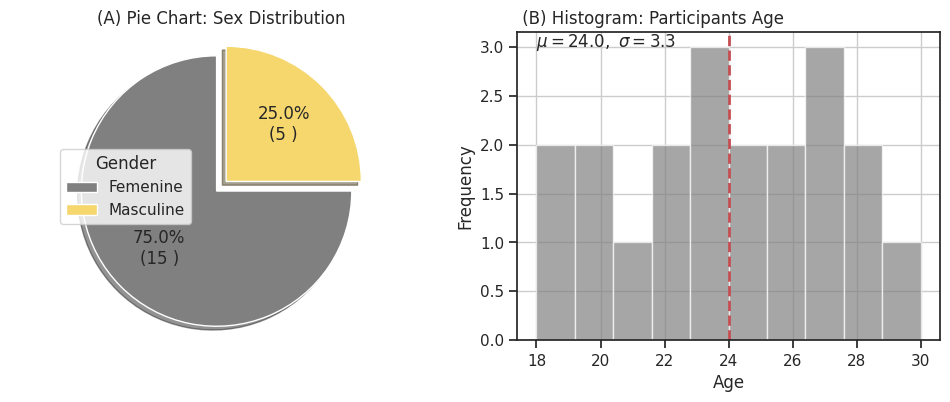
\includegraphics[width=12cm]{/home/perdices/Dokumente/Github/m-b_thesis/Analysis/figures/participants.png}
    \captionsetup{justification=justified, margin={2cm,2cm}, font={small}}
    \caption{Participants Composition}
    \label{fig:mesh1}
\end{figure}

    
\subsection*{2.2 Materials}
\subsubsection*{2.2.1 Electrocardiogram (ECG):}
Heart rate data was collected using an Arduino Uno and a SparkFun Single Lead Heart Rate Monitor - AD8232. The collected data is transferred through a USB 2.0 connection and integrated into the Unity log file at a frequency of 133 Hz. Compared to a clinical ECG, this device entails a serial interface that can send triggers via USB directly to a computer and software (e.g. Unity, Matlab) with minimal delay due to its architecture. Its software and hardware is open-source and publicly available \parencite{TimsECG}.

\subsubsection*{2.2.2 Head Mounted Display \& Lighthouses:}
The VR setup includes a HTC Vive head-mounted display (HMD) with two lighthouses. The headset specifications include a Dual AMOLED 3.6" diagonal display, with 1080 x 1200 pixels per eye (2160 x 1200 pixels combined), a 90 Hz refresh rate, and a 110-degree field of view. The lighthouses are equipped with SteamVR Tracking, G-sensors, gyroscopes, and proximity sensors. Both the HMD and lighthouses are connected using USB 2.0. For this study, the VR controllers were not used, and instead, hand tracking was performed using the Leap Motion sensor.

\subsubsection*{2.2.3 Leap Motion Controller:}
The Leap Motion Controller has a field of view of 150x120 degrees, with a variable range of roughly 80 cm (arm's length). It weighs 32 grams and is mounted on the HMD. The device features two 640x240 infrared cameras with a frame rate of 120 fps.

\subsubsection*{2.2.4 Data Gloves:}
The data gloves used in the study are equipped with magnetic sensors and connected to Unity using a microUSB connection. These gloves provide haptic feedback through 10 vibrotactile actuators, offering a wide range of tactile sensations with 1,024 levels of intensity. The gloves also incorporate complete finger tracking using six 9-axis Inertial Measurement Units (IMUs). These IMUs enable precise tracking of finger movements, allowing for accurate gesture recognition and enhanced interaction in virtual environments.

\subsection*{2.2 Materials}
\subsubsection*{2.2.1 Electrocardiogram (ECG):}
Heart rate data were collected using an Arduino Uno and a SparkFun Single Lead Heart Rate Monitor - AD8232. The collected data were transferred through a USB 2.0 connection and integrated into the Unity log file at a frequency of 133 Hz. Compared to a clinical ECG, this device entails a serial interface that can send triggers via USB directly to a computer and software (e.g. Unity, Matlab) with minimal delay due to its architecture. Its software and hardware are open-source and publicly available \parencite{TimsECG}.

\subsubsection*{2.2.2 Head Mounted Display \& Lighthouses:}
The VR setup included an HTC Vive head-mounted display (HMD) with two lighthouses. The headset specifications included a Dual AMOLED 3.6" diagonal display, with 1080 x 1200 pixels per eye (2160 x 1200 pixels combined), a 90 Hz refresh rate, and a 110-degree field of view. The lighthouses were equipped with SteamVR Tracking, G-sensors, gyroscopes, and proximity sensors. Both the HMD and lighthouses were connected using USB 2.0. For this study, the VR controllers were not used, and instead, hand tracking was performed using the Leap Motion sensor.

\subsubsection*{2.2.3 Leap Motion Controller:}
The Leap Motion Controller had a field of view of 150x120 degrees, with a variable range of roughly 80 cm (arm's length). It weighed 32 grams and was mounted on the HMD. The device featured two 640x240 infrared cameras with a frame rate of 120 fps.

\subsubsection*{2.2.4 Data Gloves:}
The data gloves used in the study were equipped with magnetic sensors and connected to softwear (Unity) using a microUSB connection. These gloves provided haptic feedback through 10 vibrotactile actuators, offering a wide range of tactile sensations with 1,024 levels of intensity. The gloves also incorporated complete finger tracking using six 9-axis Inertial Measurement Units (IMUs). These IMUs enabled precise tracking of finger movements, allowing for accurate gesture recognition and enhanced interaction in virtual environments.


\subsection*{2.3 Task}

Participants after being debiref with Covid-Specific rules, information privacy and ethical norms recieved information about the experiment. Here they cosent and proceed to do all following tasks. Important is to mention that not all task performed are used in this study. This is because this is a secondary study with a sligtly different focus from the original one. 

\begin{enumerate}
\item[(i)] \textbf{Questionnaires:} Before the IVR experience, participants completed the Edinburgh Handedness Questionnaire and the PRE-Cybersickness Questionnaire. Following the IVR experience, participants filled out the Virtual Reality Subjective Evaluation Questionnaire and POST-Cybersickness Questionnaire. Both types of questionnaires are included in the Appendix section.

\item[(ii)] \textbf{Heartbeat Count Task (HCT):} Participants performed a one-minute heartbeat count task before and after the IVR task. Note that this task is not considered within this thesis because of being out of the scope of this secondary study.
\end{enumerate}

Following the completion of the initial questionnaires and HCT, participants moved to another room where the IVR (Immersive Virtual Reality) equipment was set up. This included a head-mounted display (HMD), data gloves, and an ECG (Electrocardiogram) device. Participants received a brief training session before proceeding with the heartbeat count task and the IVR memory-motor task.


The IVR Memory-Motor Task comprised the following steps:
\begin{enumerate}
    \item[\textbf{a.}] Participants stood in front of a virtual table, allowing ample time to acclimate to the virtual environment, as depicted in Figure \ref{fig:looks}.
    
    \item[\textbf{b.}] Prior to each trial, a new calibration process started. Participants placed their palms facing up within the shadowed hands, ensuring the standard positioning. Refer to Figure \ref{fig:looks} (b) for the calibration setup.
    
    \item[\textbf{c.}] Participants viewed a two-dimensional sketch (Figure \ref{fig:looks} (c)) displayed in the virtual environment, prompting them to memorize the red ball's position. During this phase, participants kept their virtual hands open with palms facing up.
    
    \item[\textbf{d.}] The sketch disappeared, and a red ball appeared from the top, landing in either lef or right hand of the participants. As son as the ball visually touch the hand the vibration in the glove started. The vibration could match the visual location redball or not. For example, the ball in left hand vibrating glove in left hand (congruent condtion). Or ball in left hand vibration in right hand (incongruent condition). 
    
    Participants then observed a template on the table, resembling the initial sketch they memorized. Their task was to place the ball in the correct location on the template as swiftly as possible.

    \item[\textbf{e.}] After the ball is place in the template the ball and template dissapear. The complete process from a to d start again for 3 sets of 36 times. 
    
\end{enumerate}

\begin{figure}[!ht]
    \centering
    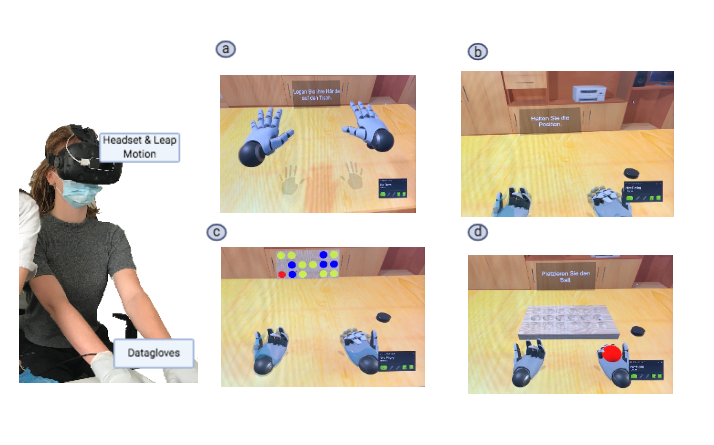
\includegraphics[width=15cm]{/home/perdices/Dokumente/Github/m-b_thesis/Analysis/figures/design_ilustration.png}
    \captionsetup{justification=justified, margin={2cm,2cm}, font={small}}
    \caption{Illustration of the IVR Memory-Motor Task: (a) represents the acclimation period during initial setup; (b) showcases the first-person perspective of the calibration phase; (c) displays the 2D sketch for memorizing ball position; (d) presents the appearance of the ball and the 3D template for ball placement, marking the beginning of each trial.}
    \label{fig:looks}
\end{figure}
 
In a sequence of 108 trials, three conditions—congruent ($V=T$), incongruent ($V \neq T$), and visual-only ($V$)—were presented randomly and rapidly, each occurring 36 times. Each trial commenced upon positioning the ball in a hand, concluding only upon its precise placement on the designated template (refer to Figure \ref{fig:looks}).

Moreover, both before and after the IVR test, participants underwent a final round of questionnaires, aiming for repetitive assessments of sickness levels. Simultaneously, initial and singular evaluations gauged the immersion experience involving the haptic glove and hands.


\subsection*{2.4 Mesurements}
\subsubsection*{2.4.1 Immersive Virtual Reality (VR):}

 Movement data from the data gloves, Leap Motion device, and the HMD was collected. For movement analysis, only the wrist movements tracked by the Leap Motion device were considered, excluding the fingertips' magnetic tracking sensor data. All movements were recorded in a Euclidean coordinate system (X, Y, Z) with the original calibrating point set at (0, 0, 0). This provided a total of nine streaming sources of data (e.g., Headset X, Headset Y, Headset Z, and so on). Notably, rotational data was not included in the analysis.

Additionally, in the game output data, there are flags that signal if a button was pressed, if the ball is placed in the holder, and when the trial started.

\subsubsection*{2.4.3 Questionnaires:}
Both of the described questionnaires are included in the appendix of this thesis for further reference.

\begin{enumerate}
\item[(i)] \textbf{Virtual Reality Subjective Evaluation Questionnaire:} This self-designed questionnaire comprises 26 items aimed at assessing the sense of reality experienced during the VR session. It explores factors like engagement level, hand movement, task difficulty, and other controlling aspects. Participants responded using a Likert scale ranging from one to seven.

\item[(ii)] \textbf{PRE/POST-Cybersickness Questionnaire:} This study employs a shortened version of the simulator sickness questionnaire (SSQ) \parencite*{avpsy}. It utilizes a Likert scale ranging from one to four, featuring labels such as "not present," "somewhat," "clearly," and "very strongly." The questionnaire consists of 16 items, gauging symptoms like "fatigue" and "general discomfort," among others.
\end{enumerate}


\subsection*{2.5 Data Analysis}

\subsubsection*{Questionnaire}
The analysis of the questionnaire responses aimed to explore the impact of haptic gloves on reported immersion and related perceptions. Initially, the raw questionnaire data collected from 20 respondents, consisting of 27 questions rated on a scale from 1 to 7, underwent meticulous processing. Missing values were checked and handled appropriately, thus leaving us with 19 respondants. Statistical analysis included the calculation of descriptive statistics such as median ($\text{Mdn}$), mean ($\mu$), and standard deviation ($\sigma$) for each question. These statistics were instrumental in understanding the central tendencies and variability in respondents' perceptions. A full view of all answers can be found in the Supplements section. 

\subsubsection*{Response Time}
We measured all response times from when the ball entered the scene in the trial until it disappeared. We excluded trials where the error button was pressed from the analysis. Before analyzing, we corrected outliers by removing data points that deviated more than 3 times the median absolute deviation (MAD), equivalent to 3 standard deviations assuming a normal distribution \parencite{Innes2019ACA}. We didn't eliminate responses for being too fast. However, we excluded 13\% of trials due to excessive slowness. The final sample included 1826 response times (approximately 24 per condition per participant). After removing outliers, we transformed the response times for each condition into rates (1/RT).

The transformation method chosen aligns with the detailed and justified steps in \cite{Innes2019ACA}, which provide more detail and justification compared to \cite{SALTAFOSSI2023108642}. Although this transformation type is contested \parencite{Lo2015-fv}, this study prioritizes normality in the error distribution over other factors, such as property scale or interacting effects, as prioritized in the referenced studies. In cases where the results were ambiguous, we also applied a General Linear Mixed-Effect Model (GLMM). The analysis diverged from the referenced studies due to mixed results, necessitating a deeper exploration of individual differences in response times while retaining the original metric. The GLMM was used for this purpose.

To allow comparisons with Saltafossi's reference paper, the primary goal was to confirm the established redundant signal effect—indicating faster response times to bimodal stimulation compared to single stimulation—and partially construct the Race model Inequality to assess its applicability across all time periods $t$.

The experimental approach followed methodologies outlined in \cite{Ulrich2007,Innes2019ACA}. Operating with one individual and two bimodal stimuli mandated a simplified version without the "bounding sum." This omission precluded the creation and analysis of the violation frontier due to the absence of the Touch alone condition, reserved for inclusion in future experimental designs.

In consideration of this, the process involved generating empirical cumulative density functions (CDFs) for three conditions—Bimodal pairs ($F_{V=T}$, $F_{V \neq T}$), and Single Signal ($F_V$). Subsequent steps included percentile determination and aggregation across participants through paired t-tests at each scrutinized percentile. For a comprehensive breakdown and reference code, consult \cite{Ulrich2007}.

\section*{3. Results}
\subsection*{3.1 Assessing the Impact of the Haptic Glove on Reported Immersion}
    
Nineteen respondents answered 27 questions, rating them on a scale from 1 (Does Not Apply) to 7 (Totally Applies). The key findings from the questionnaire are as follows:
    
\begin{enumerate}
    \item In question number 24, the perceived increase in immersion due to the haptic gloves was high ($\text{Mdn} = 6$, $\mu = 6$, $\sigma = 0.76$). Furthermore, the task was considered enjoyable at least some of the time ($\text{Mdn} = 6$, $\mu = 5.4$, $\sigma = 1.04$).
        
    \item Question 26 revealed that haptic feedback was perceived as either not significantly improving performance or having a neutral effect ($\text{Mdn} = 3$, $\mu = 3.6$, $\sigma = 1.49$). Similarly, in question 12, the perception of haptic feedback improving response time was generally rated as neutral to not applicalbe ($\text{Mdn} = 3$, $\mu = 3.7$, $\sigma = 1.74$). In question 7, when asked about the impact on results, haptic feedback was perceived as not applicable ($\text{Mdn} = 6$, $\mu = 6$, $\sigma = 0.76$).
    
    \item Notably, the assertion that it was very challenging to remember the position of the red ball ($\text{Mdn} = 2$, $\mu = 2.9$, $\sigma = 1.45$) was generally disagreed upon. Conversely, in question 8, which asked the inverse question about the ease of remembering the location of the red ball ($\text{Mdn} = 5$, $\mu = 5.1$, $\sigma = 1.37$) allign with its counterfactual. 
    
    \item The highest variance was observed in question 13 ($\text{Mdn} = 5$, $\mu = 4.2$, $\sigma = 1.79$), indicating that haptic feedback made it easier to place the ball. Similarly, question 18, which inquired about the ease of counting heartbeats at the beginning of the experiment, also showed significant variance ($\text{Mdn} = 4$, $\mu = 4$, $\sigma = 1.79$). 
        
\end{enumerate}
    
Overall, participants reported increased immersion and enjoyment as a result of the added gloves. However, there was no perceived enhancement in response attributed to the presence of the gloves. The overall task was considered easy. Moreover, the notably high variance observed in the last two questions may suggest potential confusion among participants regarding these specific queries or significant individual differences in experiences. For a more detailed breakdown, please refer to the supplementary section.
    
\subsection*{3.2 Influence of Touch Stimuli on Response Time}
\subsubsection*{3.2.1 General Performance}

First, I examined the mistake rates in ball placement per condition to ensure they did not significantly affect the experiment. The mistake rates were as follows: visual-only condition ($V$) - $6.35\%$ ($\pm 0.99\%$, SEM); visual incongruent touch condition ($V \neq T$) - $5.79\%$ ($\pm 0.59\%$); visual congruent touch condition ($V=T$) - $6.91\%$ ($\pm 1.93\%$). However, a one-way ANOVA (feedback type) showed no significant effects ($ F \leq 0.08$, $p \geq 0.91$). Despite the task's complexity beyond mere stimulus recognition, these mistake rates remained notably low and were not further analyzed.

To investigate whether the experimental manipulations mirrored the well stablished result of Redundancy Signal Effect (RSE) studies, I conducted a one-way repeated-measures ANOVA. The test revealed a significant main effect for the stimulus ($F(2,38) = 3.4$, $p \leq 0.043$, $\eta p^2 = 0.15$). The median response time for the 'Congruent' condition ($V=T$) was the fastest ($3236$ ms $\pm 456$ ms), followed by the 'Incongruent' ($V \neq T$) condition ($3268$ ms $\pm 470$), while the slowest was observed in the absence of haptic stimuli 'None' ($V$) ($3284$ ms $\pm 463$). Thus, the experimental conditions significantly influenced response times, as illustrated in Figure \ref{fig:error}.

\begin{figure}[!ht]
    \centering
    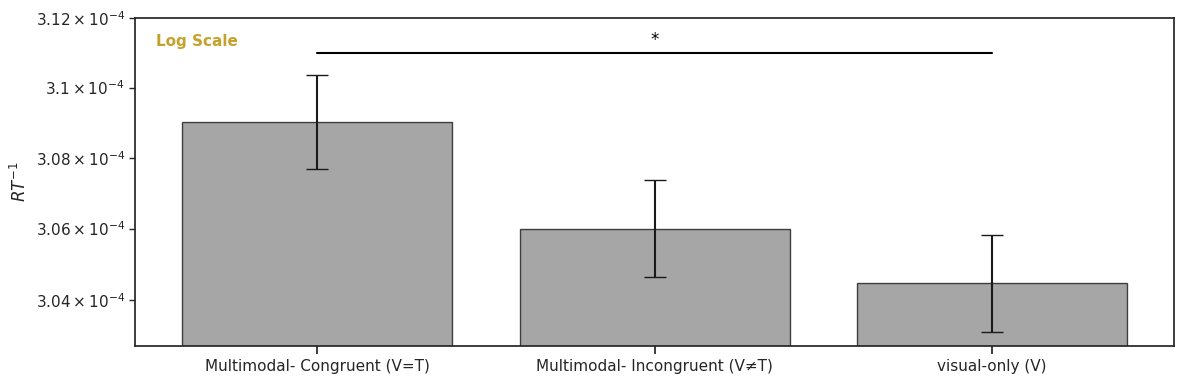
\includegraphics[width=12cm]{/home/perdices/Dokumente/Github/m-b_thesis/Analysis/figures/bar_erros_bars_stimulus_constructions.png}
    \captionsetup{justification=justified, margin={2cm,2cm}, font={small}}
    \caption{One-way repeated-measures ANOVA using $RT^{-1}$. The test revealed a significant main effect for the conditions ($F(2,38) = 3.4$, $p \leq 0.043$, $\eta p^2 = 0.15$)}
    \label{fig:error}
\end{figure}


However, post hoc Tukey HSD tests did not reveal any specific pairwise differences. While an overall difference among conditions was observed, specific pairwise differences were not identified.

Given the absence of identified specific pairwise differences in the post hoc analysis, I conducted a more comprehensive investigation using a Generalized Linear Mixed Model (GLMM). While not employed in the referenced paper, this method offers numerous advantages in multilevel research designs. It addresses the following issue stated by \textcite{Lo2015-fv}: 

"A linear relationship between the standard deviation of RTs and mean RT demonstrated in many previous studies of RT in binary choice tasks. This linear relationship is also evident in plots of the residuals, indicating heteroscedasticity in LMM analyses, characterized by an increasing spread in residuals for longer predicted RT."

As I will delve into further in the Discussion section, this issue suggests that the statistical power required for tasks involving longer Immersive Virtual Reality (IVR) times needs to be significantly higher compared to psychophysical experimental setups. An alternative approach, as mentioned by the author, is to utilize GLMM.

By using GLMM, instead of imposing normality and eliminating error deviation, we allow the use of distributions that match the properties of the measured RT \parencite{Lo2015-fv}. I utilized the \textit{statsmodels} statistical package in Python, specifically the \textit{mixedlm} function, similar to other studies \parencite{RSE_FBI}.

The mixed linear model analysis aimed to assess the impact of feedback types (($V=T$), ($V \neq T$), ($V$)) on response times. The model included feedback type as a fixed effect and participant as a random effect, with the 'Congruent' feedback type serving as the reference category.

The model coefficient for the 'None' ($V$) feedback type ($\beta = 45.726, SE = 22.594, p = 0.043$) reached statistical significance at the conventional level ($\alpha =0.05 $) when compared to the 'Congruent' ($V=T$) feedback type. This suggests a significant difference in response times between the 'None' and 'Congruent' feedback types. The coefficient for the 'Incongruent' feedback type ($\beta = 32.975, SE = 22.686, p = 0.146$) did not reach conventional levels of significance.

Thus, the 'Congruent' condition demonstrated significantly faster performance compared to the visual-only condition. This outcome aligns with the expected results according to the RSE. However, the findings present a mixed perspective. Despite this significant contrast, the more stringent post hoc Tukey HSD tests revealed no notable differences between pairwise conditions. Additionally, the GLMM indicated significance solely between the 'Congruent' and visual-only ($V=T$ - $V$) conditions and not between the 'Congruent' and 'Incongruent' conditions ($V=T$ - $V \neq T$). To understand if this mixed results are due to the irrelevancy of the 'Incongruent' condition ($V \neq T$) or the result of changed behavior over time, we can investigate the looking at our CDF analysis.

\subsubsection*{3.2.2 Race Model Inequeality}

As already mentioned in the methods section, the experiment does not allow for a full test of the RMI, since originally the experiment did not consider tactile only condition. However, I will use the CDF from the model, assess the significance of their differences, and establish comparisons among the three experimental conditions. We observed that the overall performance partially adhered to the RSE, notably between the 'Congruent' and visual-only ($V=T$ ; $V$) conditions, but no significant differences emerged between the 'Congruent' and 'Incongruent' conditions ($V=T$ ; $V \neq T$). 

To mimic the results from \Cite{SALTAFOSSI2023108642}, I conducted a series of t-tests using individual participant data for the Gx, Gy, and Gz values at each percentile level. Rather than examining areas under the curve, I focused on the raw values of Gx, Gy, and Gz. Furthermore, instead of emphasizing time bins, I opted to discuss percentile levels, given the differing time ranges compared to traditional RMI literature. 

When comparing differences between Gx and Gy ($V$ ; $V \neq T$), no significant p-values were found for any percentile. The results between Gx and Gz ($V$; $V=T$) are presented in Table \ref{tab:response-time-range}. This table illustrates the results for all time frames and percentiles. Notably, significant differences emerged between Gx and Gy from percentile 16 onwards. Interestingly, for this percentile (as depicted in Figure \ref{fig:CDF}), the single modality visual ($V$) appears to be faster than the bimodal incongruent condition ($V \neq T$), suggesting a potential violation of the RSE. Conversely, subsequent results align with our expectations from the RSE. It's essential to note that when considering the distribution of all response times, the highest density is observed between 3100 and 3200 ms, encompassing over one-third of all answered trials.
 
\begin{table}[!ht]
    \centering
    \begin{tabular}{ccccc}
    \hline
    \textbf{Gx Time Range (ms)} & \textbf{Gx Min Max Diff (ms)} & \textbf{Percentile Estimation} & \textbf{T-value} & \textbf{p-value} \\ \hline
    (3070, 3621) & 551 & 10  & 1.19 & 0.12 \\
    (3078, 3626) & 548 & 13 & 1.31 & 0.1  \\
    (3084, 3648) & 564 & 16 & 1.88 & 0.04* \\
    (3086, 3687) & 600 & 19 & 2.04 & 0.03* \\
    (3087, 3708) & 621 & 20  & 2.01 & 0.03* \\
    (3092, 3748) & 656 & 23 & 1.97 & 0.03* \\
    (3094, 3760) & 665 & 26 & 2.06 & 0.03* \\
    (3098, 3766) & 668 & 29 & 2.03 & 0.03* \\
    (3099, 3768) & 668 & 30  & 2.02 & 0.03* \\
    (3104, 3814) & 709 & 33 & 2.11 & 0.02* \\
    (3106, 3838) & 732 & 36 & 2.08 & 0.03* \\
    (3111, 3846) & 735 & 39 & 1.83 & 0.04* \\
    (3114, 3848) & 734 & 40  & 1.79 & 0.04* \\
    (3119, 3861) & 741 & 43 & 1.74 & 0.05* \\
    (3121, 3907) & 786 & 46 & 1.55 & 0.07  \\
    (3123, 3969) & 846 & 49 & 1.36 & 0.09  \\
    (3124, 3978) & 855 & 50  & 1.33 & 0.1   \\
    (3130, 4171) & 1041 & 60  & 1.25 & 0.11  \\
    (3141, 4352) & 1211 & 70  & 1.21 & 0.12  \\
    (3153, 4645) & 1492 & 80  & 1.47 & 0.08  \\
    (3176, 4948) & 1772 & 90 & 0.53 & 0.3   \\ \hline
    \end{tabular}
    \captionsetup{justification=justified, margin={2cm,2cm}, font={small}}
    \caption{T-test results between Gx \& and Gz conditions. Response Time Range (ms), Difference RT (ms), Percentile Estimation, T-value, and p-value for each Percentile using the results of t-tests. * indicates significant p-values.}
    \label{tab:response-time-range}
\end{table}


\begin{figure}[!ht]
    \centering
    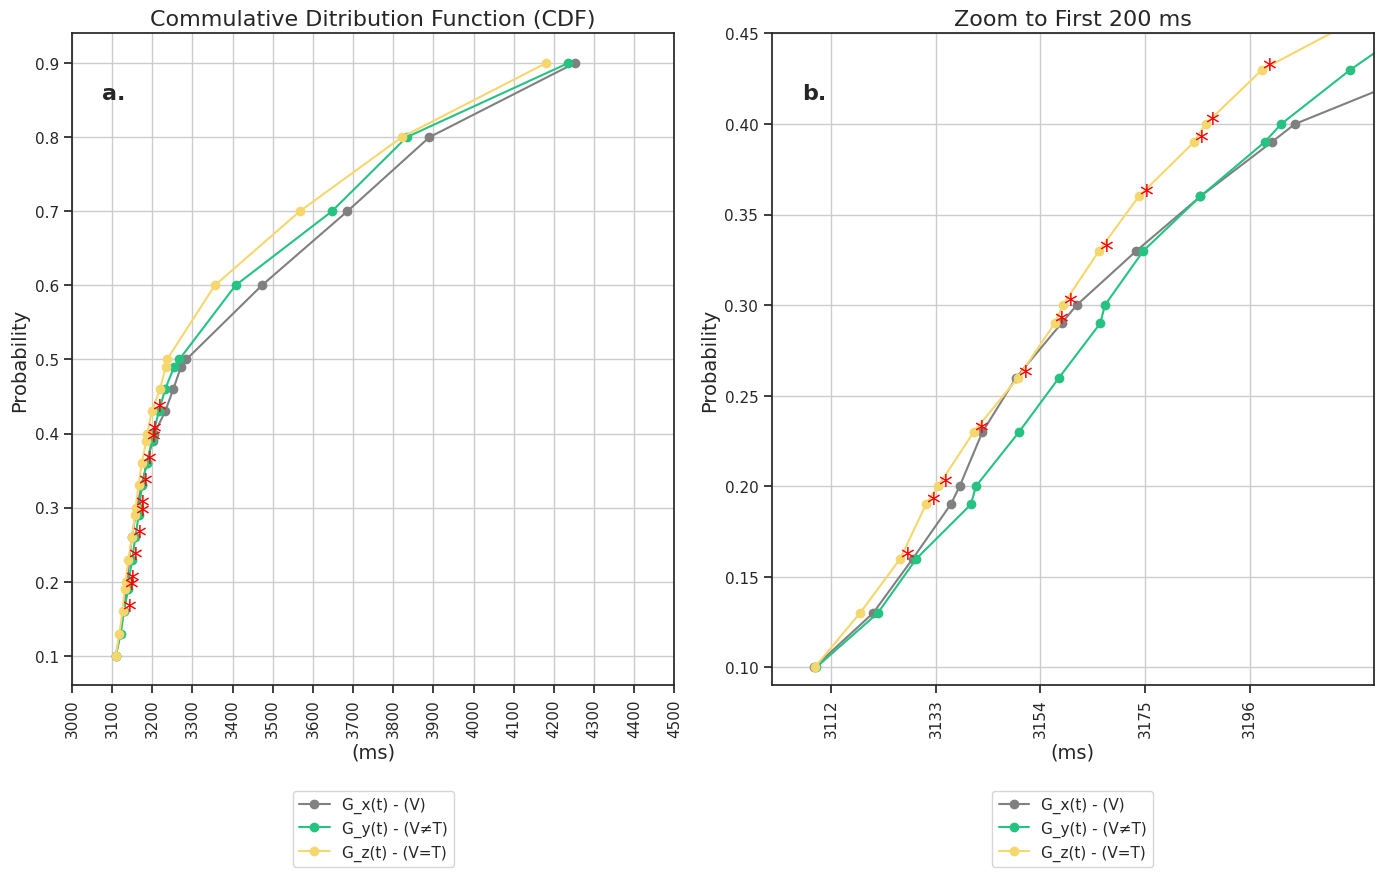
\includegraphics[width=15cm]{/home/perdices/Dokumente/Github/m-b_thesis/Analysis/figures/CDF.png}
    \captionsetup{justification=justified, margin={2cm,2cm}, font={small}}
    \caption{ (a.) Displays the 10 estimated percentile points for each of the three functions of interest: Gx, Gy, Gz, considering all participants. (b.) Is a zoom in the first 100 ms. Acording to the RSE, the visual $V$ type should be under Gy, Gz at all moments. Our data shows that is not the case for the RT in the first 200 ms.}
    \label{fig:CDF}
\end{figure}


\section*{4. Discussion}

This thesis aimed to test the feasibility of using IVR to study how the cardiac cycle modulates cognition and to bridge the gap between cognitive and psychophysical research. To achieve this goal, the thesis used an IVR memory task where participants had to remember a location and immediately place a red ball over this location in a 3D template. The condition was desgined so that  a passive vibro-tactile stimuli was activated along with the ball being presented into either matching the visual location of the ball or in the opposite hand. The study employed a within-subject experimental design with three categories: congruent visual-tactile stimuli, incongruent visual-tactile stimuli, and visual-only stimuli. The measured parameters were Reaction Time (RT) and Accuracy.

To establish a comparison, I followed the steps outlined in my reference study \parencite{Innes2019ACA, SALTAFOSSI2023108642, Ulrich2007}. It's important to note that there is only a single modality stimuli ($V$), limiting the possibilities of RMI comparisons.

The initial step involved testing the validity of stimulus construction by analyzing and modeling reaction times to uni-modal and bi-modal stimuli. Results were mixed. Overall, a significant difference between the conditions existed. While attempting to identify pairwise differences through a Tukey HSD test, no significant differences were found. However, a GLMM showed a significant difference between the visual-only ($V$) and visual-touch congruent ($V=T$) conditions. No significant differences were found between the incongruent ($V \neq T$) and the visual-only ($V$) conditions. These results confirmed the well-observed RSE in virtual reality during a ball positioning task and raised questions about the incongruent condition.

Analyzing the RMI reveals that the most frequently occurring RT falls between 3100 ms and 3200 ms, with over one-third of all trials within this 100 ms range. Additionally, when performing a t-test for all participants, the cumulative functions for each condition (Gx and Gz values) were significantly different only within this 100 ms period, not before or after. It's important to note that although the difference between Gx and Gy was not significant, for this 100 ms period, a potential violation of the RSE principle was observed, where a bimodal condition ($V \neq T$) was slower than a unimodal condition ($V$).

Descriptively, the same relationship between the visual-only ($V$) and the congruent condition ($V=T$) holds throughout the entire range of RT, in accordance with the RSE. However, this is not the case for RT between the incongruent condition and the visual-only condition, where the visual-only condition is faster than the incongruent condition ($V \neq T$) for the first 100 ms of the trial, violating the RSE. Later, the incongruent condition is faster than the unimodal visual-only condition, as expected with the RSE.

\Cite{RSE_FBI} proposes a plausible explanation for the absence of a difference in the RSE between congruent and incongruent conditions. It suggests that the mere simultaneous occurrence of visual and vibrotactile stimuli might suffice for multisensory integration, irrespective of whether these multisensory stimuli are functionally linked at a higher level or not (e.g., touch in the hand holding the ball).

An alternative explanation may relate to the context invariance assumption, which states that the processing of one signal is not affected by another.

The discrepancy observed in the incongruent case may be so marginal that the statistical power of the present study might not be sufficient to detect it significantly. Regarding the power of the study, one conclusion is that, due to considerations of ecological validity, each trial in our IVR study spans a longer time frame compared to traditional psychophysics experiments (with a mean duration of 3400 ms as opposed to the typical 200 ms). This extended duration contributes to increased variance and skewness in response times (RT). Moreover, according to the literature, the influence of the cardiac cycle on stimuli ranges from 10 to 40 ms, posing a challenge when investigating its effects in IVR environments. Consequently, the statistical power of future research needs to be increased threefold, considering, for instance, involving 60 participants, especially if an additional condition related to cardiac cycles is to be included in the analysis.



\newpage
\section*{Supplement}
    \begin{figure}[H]
        \centering
        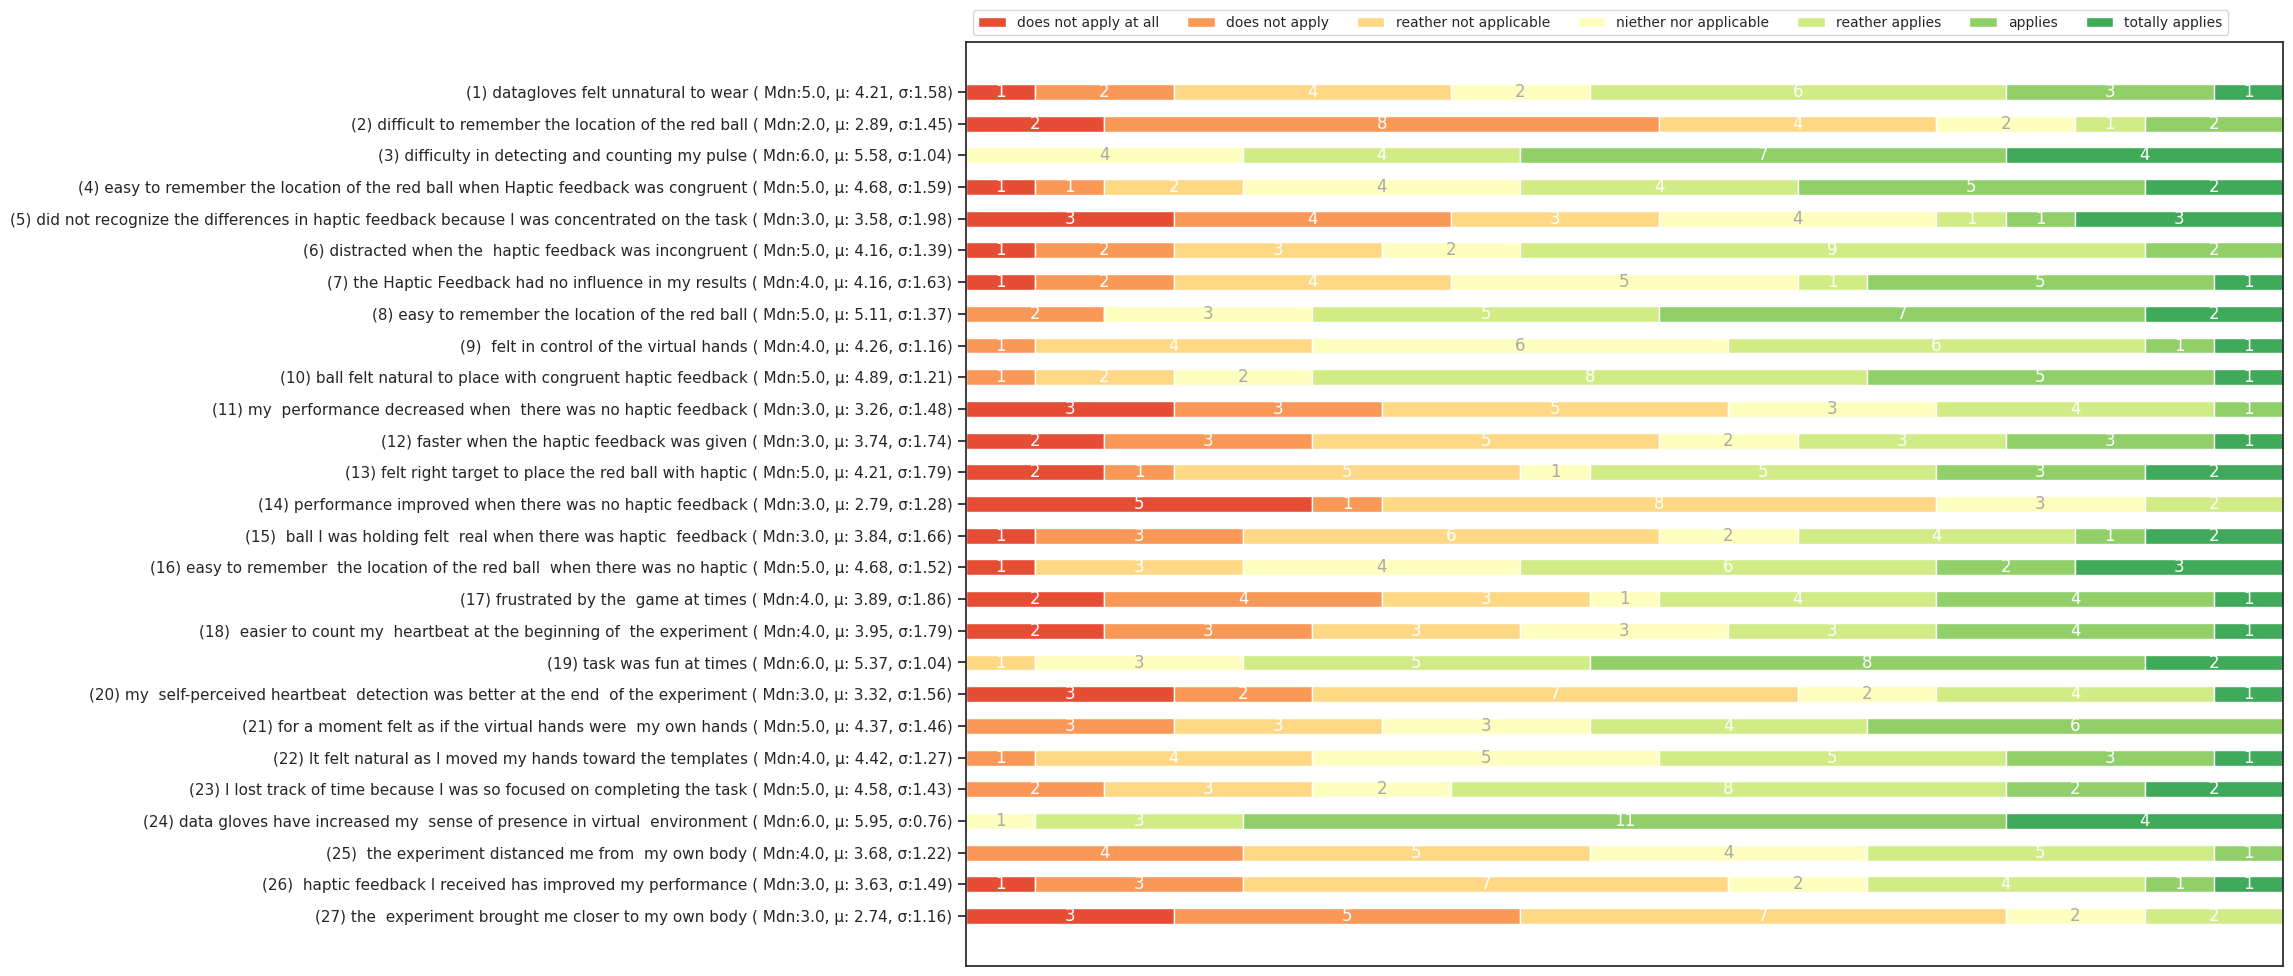
\includegraphics[angle=90, width=\textwidth, height=20cm, keepaspectratio]{/home/perdices/Dokumente/Github/m-b_thesis/Analysis/figures/questionaire_fig.png}
        \captionsetup{justification=justified, margin={2cm,2cm}, font={small}}
        \caption{Results: Virtual Reality Subjective Evaluation Questionnaire}
        \label{fig:quest}
    \end{figure}
\pagebreak


%-------- CREATING BIBLIOGRAPHY

\paragraph{\textbf{References}}
\printbibliography[heading=none]

%-------- CREATING Apendix

\pagebreak
\vspace*{\fill}
\section*{\centering Additional Material}
\vspace*{\fill}



\end{document}

